\documentclass{beamer}

%\usepackage{subfigure}
\usepackage{graphicx}
\usepackage{sidecap}
\usepackage{caption}
\usepackage{subcaption}
\captionsetup{compatibility=false}
\usepackage{appendixnumberbeamer}
\usepackage{amsmath}
% --
\usepackage{multirow}
\usepackage{xcolor}
\usepackage{setspace}
\usepackage{hyperref}
\usepackage{anyfontsize}

\setbeamertemplate{footline}

\newenvironment{itemise} {\begin{itemize} \setlength{\itemsep}{0.2cm}} {\end{itemize}}
\usepackage[labelformat=empty]{caption}
\setbeamertemplate{sections/subsections in toc}[square]

%% COLORS
\definecolor{Gray}{gray}{0.9}
\definecolor{dblue}{rgb}{0.132,0.1,0.27}
\definecolor{mint}{cmyk}{1.0, 0.2, 0.6, 0.05}
\definecolor{ant}{cmyk}{0.5, 0.1, 0.0, 0.45}
\definecolor{lgray}{cmyk}{0.12, 0.0, 0.0, 0.17}
\definecolor{lred}{cmyk}{0.0, 0.9, 0.7, 0.0}


\usepackage{etoolbox}% http://ctan.org/pkg/etoolbox 
\usepackage{booktabs}

\newenvironment{literatur}{%
  \parskip2pt \parindent0pt \raggedright
  \def\lititem{\hangindent=0.5cm \hangafter1}}{%
  \par\ignorespaces}

\newcommand{\tb}[1]{{\color{blue}{\textbf{#1}}}}
\newcommand{\tm}[1]{{\color{mint}{\textbf{#1}}}}
\newcommand{\tr}[1]{{\color{red}{\textbf{#1}}}}
% Ilya: packages

\usepackage{tikz}
\usepackage{lmodern}
\usepackage{enumitem}

% Ilya: my commands

\newenvironment{mytemize}
{\vfill\itemize[nolistsep,itemsep=\fill,label=\color{blue}{$\triangleright$}]}
  {\enditemize}


\newenvironment{mynumerate}
{\vfill\enumerate[nolistsep,itemsep=\fill,label=\arabic*.]}
  {\endenumerate}

\newcommand{\hitem}[1]{
  {\color{blue}{$\triangleright$}} 
  {#1} 
  {\hfill}
}

\setlist[itemize]{label= \color{blue}{$\triangleright$}}
\setlist[enumerate]{label = \arabic*.}

\newcommand{\rarr}{$\Rightarrow$\ }

%------------------------------------------------------------------------------------
% TITLE
%------------------------------------------------------------------------------------
\title[PSME]{Macroeconomics\\ Lecture 12 -- Fiscal Policy}
\author[I. Eryzhenskiy]{Ilya Eryzhenskiy}
\institute[Paris-1]{PSME Panth\'{e}on-Sorbonne Master in Economics}
\date[PSME macro]{Fall 2022}

%---BEGIN------------------------------------------------------------------------------
\begin{document}
%---BEGIN------------------------------------------------------------------------------
\begin{frame}
\maketitle
\end{frame}
%---FRAME------------------------------------------------------------------------------
%\section{Outline}
\begin{frame}
\frametitle{Outline}
\tableofcontents
\end{frame}

\section{Government budget sustainability}

\begin{frame}{Government budget constraint}
  Denote real net government asset position at beginning of period $t$ as $B^g_t$. \\
  Typically, $B_t^g<0$ \rarr introduce a \tb{government debt} variable $D_t = -B^g_t$. \\
\vfill
The government budget constraint can be written with the same logic as for household:  
  \begin{align*}
	G_t + B^g_{t+1} - B^g_t &= r_{t} B^g_t + T_t \\
	\text{or} \quad G_t - D_{t+1} + D_t &= - r_{t} D_t + T_t  \\
  \Leftrightarrow  \quad D_{t+1} - D_t &=  \underbrace{\underbrace{r_{t} D_t}_{\text{\tb{debt service}}} + \underbrace{G_t - T_t}_{\text{\tb{primary deficit}}}}_{\text{\tb{total deficit}}} \\
	\Leftrightarrow \quad D_{t+1} &= D_t (1+r_{t}) + G_t - T_t
  \end{align*}
  Last equation -- \tm{recursive} (as many others in course) \rarr can write it as an infinite sum.
\end{frame}

\begin{frame}{Government budget sustainability}
  $$D_t = \sum_{k=0}^{\infty} \frac{T_{t+k} - G_{t+k}}{R_{t, t+k}} + \underbrace{\lim_{\to\infty}\frac{D_{t+k}}{R_{t, t+k}}}_{=0}$$
  where $R_{t,t+k} \equiv (1+r_t)\cdot(1+r_{t+1}) \cdot (1+r_{t+2})\cdot \dots (1+r_{t+k}) = \Pi_{s=0}^k (1+r_{t+s})$ and last term being null is transversality condition.
  \begin{mytemize}
  \item Future \tb{primary surpluses} must be used to repay initial government debt 
  \item The earlier primary surplus in the future, the more impact on debt dynamics
  \item \textbf{Interest rates matter} \rarr in short term with sticky prices, pressure on Central Bank from government. Another reason for independent status of CB  with inflation targeting mandate
  \end{mytemize}
\end{frame}

\section{Ricardian equivalence}
\begin{frame}
\frametitle{Outline}
\tableofcontents[currentsection]
\end{frame}
\begin{frame}{Government budget and private budget}
Consider a flow budget constraint of an infinitely lived household:
$$ C_t + \Omega_{t+1} - \Omega_t = w_t L_t + r_t \Omega_t + \Pi_t \textcolor{blue}{- T_t}$$
$$ \Omega_{t+1} = (1+r_t) \Omega_t +  w_t L_t + r_t \Omega_t + \Pi_t \textcolor{blue}{- T_t}- C_t $$
Write as infinite sum, using same algebra:
$$\Omega_t = \sum_{k=0}^{\infty} \frac{C_{t+k} - w_{t+k} L_{t+k} - \Pi_{t+k}}{R_{t, t+k}} + \sum_{k=0}^{\infty} \frac{T_{t+k}}{R_{t, t+k}}+ \underbrace{\lim_{k\to\infty}\frac{\Omega_{t+k}}{R_{t, t+k}}}_{=0}$$
And use $\sum_{k=0}^{\infty} \frac{T_{t+k}}{R_{t, t+k}} = D_t + \sum_{k=0}^{\infty} \frac{G_{t+k}}{R_{t, t+k}}$ (from government b.c.) in the equation:  
$$\Omega_t = \sum_{k=0}^{\infty} \frac{C_{t+k} - w_{t+k} L_{t+k} - \Pi_{t+k}}{R_{t, t+k}} + \sum_{k=0}^{\infty} \frac{G_{t+k}}{R_{t, t+k}}+ D_{t}$$
\end{frame}

\begin{frame}{Budget constraints combined: Ricardian equivalence}
  Write consumptions on the left and incomes, initial assets, government spending on the right:
  $$\sum_{k=0}^{\infty} \frac{C_{t+k} }{R_{t, t+k}} = \Omega_t - D_t  + \sum_{k=0}^{\infty} \frac{ w_{t+k} L_{t+k} + \Pi_{t+k}\textcolor{red}{- G_{t+k}}}{R_{t, t+k}} $$
\begin{mytemize}
\item The expression summarizes the budget constraint of the household
\item Because of the government budget constraint, it does not depend on values of taxes 
\item Initial gov. debt, $D_t$, appears in the constraint, but its difference with $\Omega_t$ is fixed (see below)
\item[\rarr] \textbf{Given a sequence of future government expenditures} $\{G_t \}_{t=0}^\infty$, \textbf{it is irrelevant for agents' decisions how it is financed: timing of taxes and debt issuance.}
\end{mytemize}
\end{frame}

\begin{frame}{Ricardian equivalence: gov. debt vs. private wealth}
  We will now show that the $\Omega_t - D_t$ difference is always fixed. \\
  \vfill
  Suppose in $t-1$ the government decided, to tax current generations less and to borrow more instead: $\Delta D_t = -\Delta T_{t-1}$. This is under \textbf{fixed} $\{G_{t-1+k}\}_{k=0}^\infty$. 
  Reaction of household in $t-1$: 
	\begin{mytemize}
	\item a \tm{positive income shock} $- \Delta T_{t-1} >0$, but \tr{it must be temporary} because of gov. budget constraint 
	\item the change in fiscal policy is just shifting income in time: \tm{increase} of current income by \tm{$-\Delta T_{t-1}$} at $t-1$, but must \tr{decrease} future income by \tr{$\frac{\Delta T_{t-1} }{ R_{t-1, s}}$} at some future date $s$ to respect gov. budget constraint
	\item \textbf{same income shifting achieved by private savings} \rarr if household decreases savings $\Omega_t - \Omega_{t-1}$ by same amount, it keeps its optimal consumption plan $\{C_{t-1+k}\}_{k=0}^\infty$
	\item we get that $\Delta \Omega_t = \Delta D_t$, so $\Omega_t - D_t$ fixed and not affected by how the government finances $\{G_{t-1+k}\}_{k=0}^\infty$.
	\end{mytemize}
\end{frame}
\begin{frame}{Ricardian equivalence in various models}
  The result holds universally in economies that have infinitely lived households, lump-sum taxation and no market frictions. Consider 3 classes of RBC models:
  \begin{mynumerate}
  \item Closed economy without capital (see flex-price NK): \tb{$\Omega_t = D_t$} must always hold (nowhere to invest apart gov. debt). $\Delta \Omega_t = \Delta D_t$ holds trivially.
  \item Closed economy with capital (vanilla RBC): $\Omega_t - \Omega_{t-1} = I_t + D_t - D_{t-1}$, so $\Delta \Omega_t = \Delta D_t$ \rarr \tb{$\Delta I_t = 0$}.
  \item Open economy RBC: $\Omega_t - \Omega_{t-1} = I_t + IIP_t - IIP_{t-1} + D_t - D_{t-1}$. \\$\Delta \Omega_t = \Delta D_t, \Delta I_t = 0$ \rarr \tb{$\Delta IIP_t = \Delta CA_t = 0$}.
  \end{mynumerate}
\end{frame}

\section{RBC with government}
\begin{frame}
\frametitle{Outline}
\tableofcontents[currentsection]
\end{frame}
\begin{frame}{RBC with government}
  Consider a closed economy RBC with a government. Household has 2 ways to do savings: renting capital to firms with a rental rate $R_t$ and hold governemnt bonds that pay real interest $r_t$: 
\begin{align*}
  \max _{C_{t}, L_{t}, K_{t+1}, B_{t+1}} &E_{0} \sum_{t=0}^{\infty} \beta^{t}u(C_{t}, L_{t}, \textcolor{purple}{G_t}) \\
\text { s.t. } \ \
C_{t}+I_t+D_{t+1} &=  w_{t} L_{t}- T_t +R_{t} K_{t} +\Pi_{t}+(1+r_{t}) D_{t} \\
K_{t+1} &= (1-\delta)K_t + I_t \\
D_{t+1} &= (1+r_t) D_t + G_t - T_t
\end{align*}
\end{frame}
\begin{frame}{RBC with government -- closing the model}
  Preferences: 
  \begin{mytemize}
  \item 	Assume $u(C_{t}, L_{t}, G_t)$ \tb{additively separable} in $(C_t, L_t)$ and $G_t$
\begin{mytemize}
\item e.g. $\frac{C_t^{1-\sigma}}{1-\sigma} - \frac{L_t^{1+\xi}}{1+\xi} + \frac{\textcolor{purple}{G_t}^{1-\gamma}}{1-\gamma}$
\end{mytemize}
  \item Then $u'_C, u'_L$ don't depend on $G_t$ \rarr \textbf{no effect on behavior} \\
  \end{mytemize}
\vfill Production: 
\begin{mytemize}
\item $Y_t = Z_t f(K_t, L_t) = C_t + I_t + G_t$; 
\item Firm FOC: $Z_t f'_K(K_t, L_t) = R_t$;\quad  $Z_t f'_L(K_t, L_t) = w_t$
\end{mytemize}

\vfill Two independent stochastic variables now: $Z_t, G_t$: 
\begin{mytemize}
\item $\ln Z_t = \rho_z \ln Z_{t-1} + \epsilon^z_t$ 
\item $\ln G_t = (1-\rho_g)\ln(\omega Y)+\rho_g \ln G_{t-1} + \epsilon^g_t$ \rarr $G = \omega Y$ in s.s.
\end{mytemize}
\end{frame}

\begin{frame}{Effect of government spending on consumer}
  Use $D_{t+1} = (1+r_t) D_t + G_t - T_t$ in the household's budget constraint:
  \begin{align*}
	C_{t}+I_t\textcolor{purple}{+D_{t+1}} &=  w_{t} L_{t}\textcolor{purple}{- T_t} +R_{t} K_{t} +\Pi_{t}+\textcolor{purple}{(1+r_{t}) D_{t}} \\
	C_{t}+I_t &=  w_{t} L_{t}\textcolor{purple}{- G_t} +R_{t} K_{t} +\Pi_{t}
  \end{align*}
  Both debt and taxes disappear altogether from the constraint, only \textcolor{purple}{$G_t$} matters -- this is Ricardian equivalence.
\vfill
The effect of an increase of $G_t$ is then same as a negative income shock from consumer perspective:
\begin{mytemize}
\item Use intuition on consumption smoothing to understand response of $C_t, I_t$
\item Persistence of $G_t$ (parameter $\rho_g$) $\sim$ temporary vs. permanent income shocks
\item Response of $Y_t$ more ambiguous since $Y_t = C_t + I_t +\textcolor{purple}{G_t}$ 
\end{mytemize}
\end{frame}

\begin{frame}{Impulse responses -- positive shock of G}
  Cobb-Douglas production,  $u(C_t, L_t, G_t) = ln C_t - \theta \frac{L_t^{1+\chi}}{1+\chi} + \frac{G_t^{1-\gamma}}{1-\gamma}$ and 
  \centering
  \begin{tabular}{|c|c|c|c|c|c|c|c|}
	\hline
  $\alpha$ & $\beta$& $\chi$ & $\delta$& $\theta$ & $\rho_a$& $\rho_g$&$\omega$ \\
	\hline
  1/3 & 0.99 & 1 & 0.025 & 4 & 0.97 & 0.95 & 0.2 \\
	\hline
  \end{tabular}
  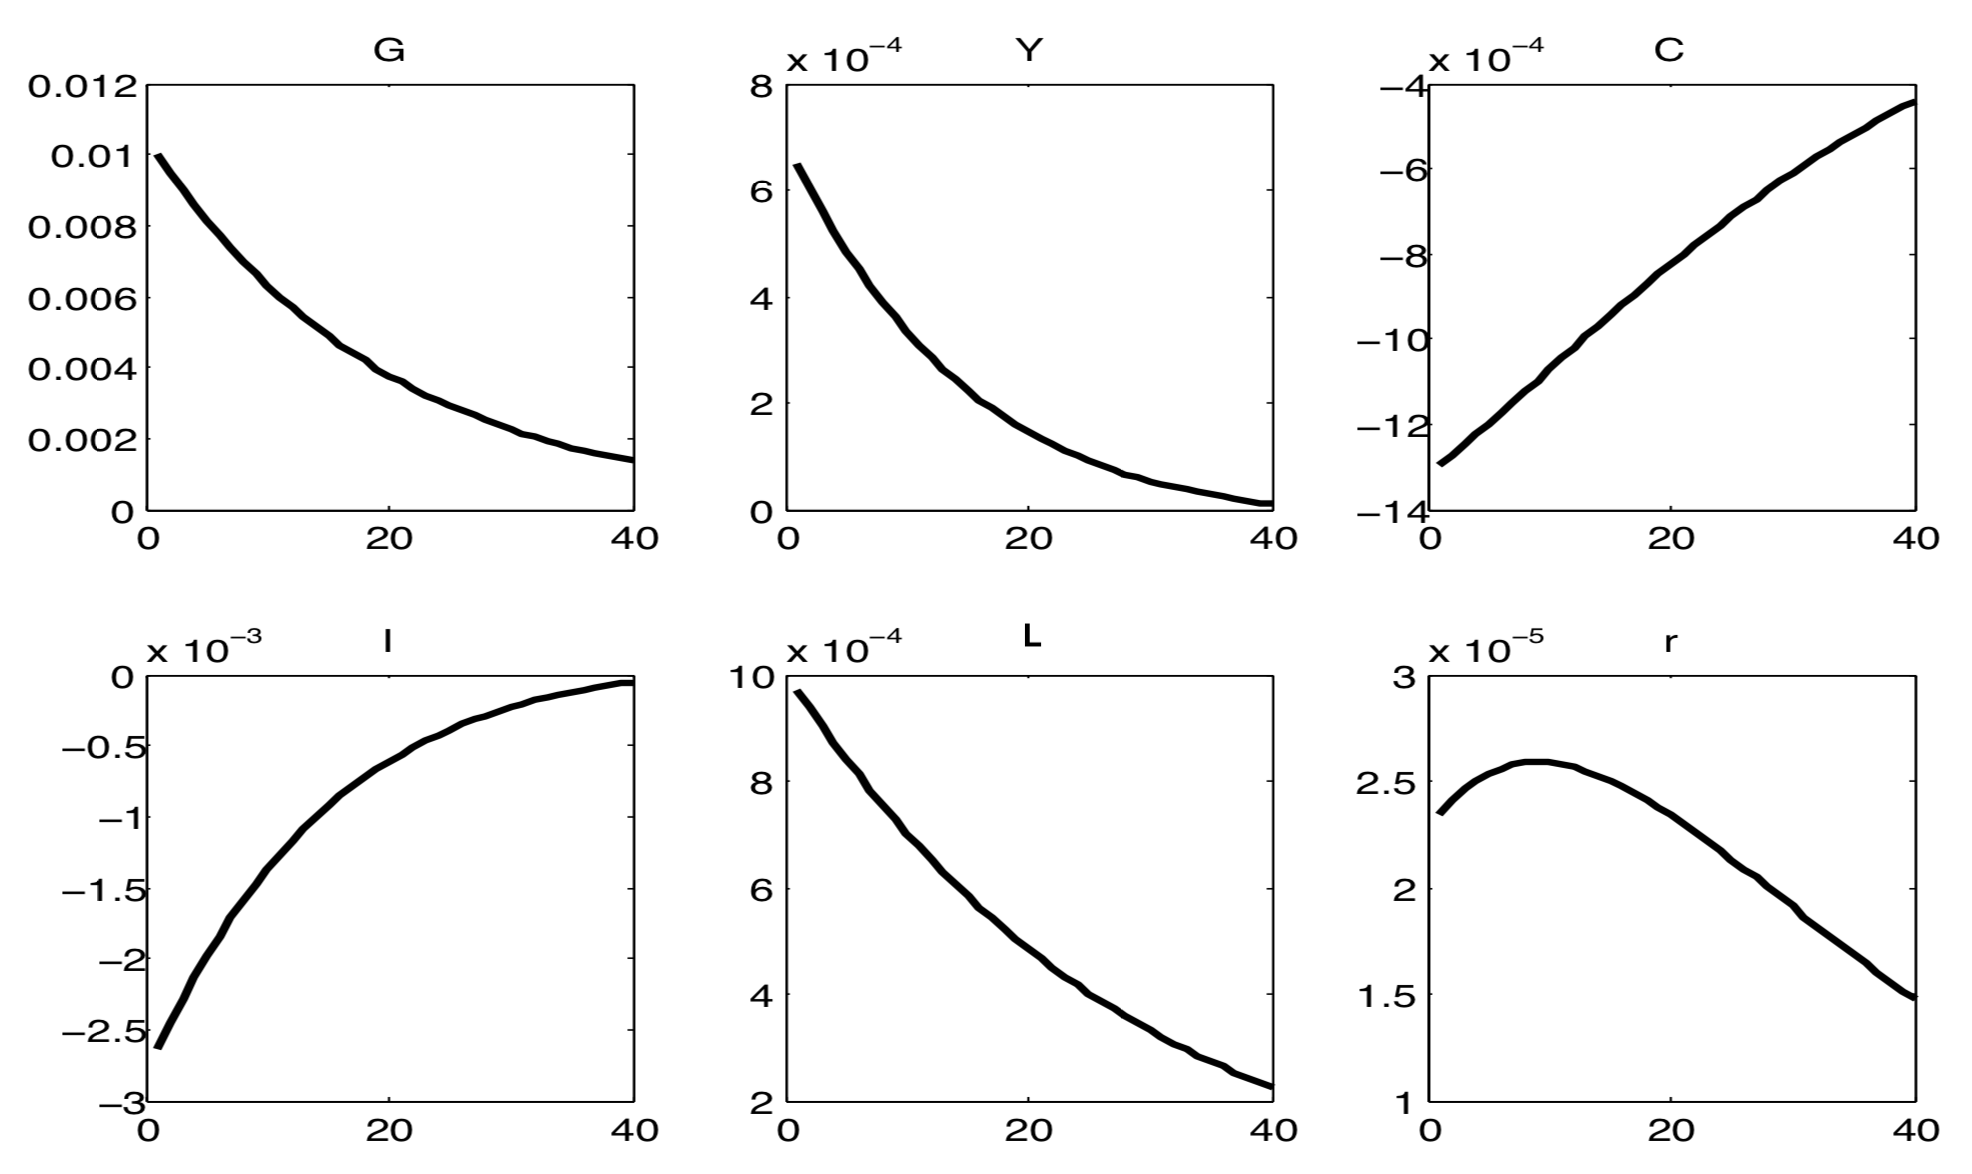
\includegraphics[width = 0.9\textwidth]{FIGURES/G_RBC_IRF.png}
\end{frame}

\section{Distortionary taxes}
\begin{frame}
\frametitle{Outline}
\tableofcontents[currentsection]
\end{frame}
\subsection{Aggregate distortions: tax smoothing}
\begin{frame}
\frametitle{Outline}
\tableofcontents[currentsubsection]
\end{frame}
\begin{frame}{Distortionary taxes}
  Lump-sum taxes is a simplifying assumption that leads to a surprising result of Ricardian equivalence.
  \vfill
  Proportional taxes \rarr strong effects on equilibrium and \tb{welfare}.
  \vfill 
  Consider labor taxation. Disposable income of household is $(1-\tau^L_t)w_t L_t$. When used in a standard consumption leisure choice, one gets: 
  $$ \frac{u'_L(C_t, L_t)}{u'_C(C_t, L_t)} = \textcolor{purple}{(1-\tau^L_t)}w_t$$
  Take example of GHH utility: $ u(C_t,L_t) = \frac{\left( C_t-L_t^{\chi}/\chi \right)^{1-\sigma} -1 } {1-\sigma}$ where $\chi>1$ \rarr 
  $ L_t = ((1-\tau^L_t)w_t)^{\frac{1}{\chi-1}} $ -- negative effect on labor supply, \rarr proportional tax \textbf{affects behavior}
\end{frame}

\begin{frame}{Tax distortions}
  $$ \frac{u'_L(C_t, L_t)}{u'_C(C_t, L_t)} = \textcolor{purple}{(1-\tau^L_t)}w_t$$
  Proportional taxes are viewed as \textit{wedges} in welfare analysis: they make \textbf{marginal rates of substitution/transformation} differ from \textbf{market prices}. 
\vfill
\rarr First Welfare Theorem does not hold: equilibrium is not optimal.  
\vfill Aim of social planner is now to \textbf{minimize distortions} induced by taxes, while financing public expenditure.
\end{frame}

\begin{frame}{Tax smoothing: a simple model}
  Consider a stylized (i.e. highly simplified) model of a social planner that chooses an aggregated tax rate $T_t/Y_t$ every period. 
\vfill
The only aim is to minimize distortions that are given by $Y_t \xi(T_t/Y_t)$ with $\xi(0) = 0; \xi'(\cdot)>0, \xi''(\cdot)>0$ a concave distortion function. Convexity of the distortion function is obtained in various  models when losses of utility are analyzed.
  \begin{align*}
	\min_{\{T_{t+k}/Y_{t+k}\}_{k=0}^\infty} E_t &\sum_{k=0}^\infty \frac{Y_{t+k} \xi(T_{t+k}/Y_{t+k})}{R_{t,t+k}} \\
	\text{s.t.} \quad D_t &= E_t \sum_{k=0}^\infty  \frac{T_{t+k} - G_{t+k}}{R_{t,t+k}}
  \end{align*}
\end{frame}

\begin{frame}{Tax smoothing -- solution}
  The FOC is $\xi'(T_t/Y_t) = E_t \xi'(T_{t+1}/Y_{t+1})$. \vfill In a deterministic model, this means $T_t/Y_t$ must be constant, so that \tb{tax distortions are smoothed} across periods. 
  \vfill For a model with uncertainty, one can further assume $\xi(\cdot)$ is quadratic \rarr $\xi'(\cdot)$ is linear \rarr the FOC becomes 
  $$\xi'(T_t/Y_t) = \xi'(E_t T_{t+1}/Y_{t+1}) \Leftrightarrow T_t/Y_t = E_t [T_{t+1}/Y_{t+1}]$$
  \rarr changes in tax rate only happen due to unexpected shocks.
\end{frame}

\begin{frame}{Tax smoothing and government debt}
  Government debt provides a ``buffer'' role when taxes need to be smoothed:
  \begin{mytemize}
  \item In periods with above-average spending needs (positive shock of $G_t$), issue additional debt not to tax too much 
  \item In periods with below-average spending needs, additional budget surplus used to finance debt repayment.
  \end{mytemize}
\end{frame}
\subsection{Taxing multiple goods: the Ramsey problem}
\begin{frame}
\frametitle{Outline}
\tableofcontents[currentsubsection]
\end{frame}
\begin{frame}{The Ramsey problem}
  We now focus on a \tr{static} problem of choosing which goods to tax at which rate.
\vfill
  Main result is the \tb{Ramsey taxation rule}: \textbf{the higher the elasticity of demand of a good for the household, the lower the optimal tax rate on that good.}
  \vfill 
  \underline{Intuition}: proportional tax raises consumer prices; consumers' reaction higher if elasticity higher. More reaction \rarr more \tr{distortions} with respect to the optimal equilibrium without proportional taxes.
\vfill
  The solution of the model will also show the \tb{primal approach} to optimal policy solution, widely used for macro models.
\end{frame}
\begin{frame}{The Ramsey problem: framework}
  $N$ goods in the economy, produced with a linear production function using labor only: 
  $$y_i = a_i l_i$$ 
  The social planner needs to finance a set of public goods $\{g_i\}_{i=1}^N$ and can only do it with proportional taxes on consumption of the goods: $\{\tau_i\}_{i=1}^N$. Think of a set of VATs.
  \vfill
  The household consumes all the goods and provides labor. Utility function: 
  $$U(c_1, c_2,\dots c_N) = \sum_i u(c_i) - \theta l$$
  Firms make zero profits on each good: \\ $\Pi_i = p_i a_i l_i - l_i = 0 \Leftrightarrow$ \tm{$p_i = 1/a_i$} \\
  Finally, goods and labor markets clear: $y_i = c_i + g_i$; $\sum_i l_i = l \Leftrightarrow \sum_i \frac{y_i}{a_i} = l \Leftrightarrow$ \tm{$\sum_i \frac{c_i+g_i}{a_i} = l$}
\end{frame}

\begin{frame}{Household problem}
  \begin{align*} 
	\max_{\{c_i\}, l}\sum_i &u(c_i) - \theta l \\
	\text{s.t.} \ \ &\sum_i (1+\tau_i) p_i c_i = l
  \end{align*}
  The FOCs are $u'(c_i) - \lambda (1+\tau_i)p_i=0$ and $\lambda = \theta$. Combining, \tm{$u'(c_i) = \theta p_i (1+\tau_i)$}. \\
  \tm{Isoelastic} form of utility from consumption: \tm{$u(c_i) = \frac{c^{1-\frac{1}{\varepsilon_i}}}{1-\frac{1}{\varepsilon_i}}$}. \\ Note that each good has its own parameter $\varepsilon_i$.
  \vfill The FOC then becomes: $$ c_i = (\theta (1+\tau_i) p_i)^{-\varepsilon_i}$$
  We can now see that $\varepsilon_i$ is the \tb{demand elasticity}. Another useful interpretation is $\varepsilon_i = \frac{u''(c_i) c_i}{u'(c_i)}$. 
\end{frame}

\begin{frame}{Primal approach to optimal taxes}
  We can rewrite the consumer's budget constraint using the FOC:
  $$ \sum_i u'(c_i) c_i = \theta l $$
  This is called the \tb{implementability constraint} -- an optimality condition for HH choices where prices are eliminated. \\
  \vfill
  The \tb{primal approach} to finding optimal taxes:  
  \begin{mynumerate}
  \item 	
  use the implementability constraint in the social planner's optimization and solve for optimal consumption
\item use budget constraints and FOCs to find taxes that yield the optimal consumption
  \end{mynumerate}
\end{frame}

\begin{frame}{Primal approach -- social planner's problem}
  \begin{align*} 
	\max_{\{c_i\}, l}\sum_i &u(c_i) - \theta l \\
	\text{s.t.} \ \ &\sum_i u'(c_i) c_i = \theta l \quad &\text{implementability constraint}\\
	 &\sum_i \frac{c_i+g_i}{a_i} = l\quad &\text{resource constraint}
  \end{align*}
  Lagrangian needs to have two multipliers. \\
  \vfill
  Manipulate the FOCs to eliminate both multipliers an get  relationship between tax rates of two goods and their demand elasticities $\frac{u''(c_i) c_i}{u'(c_i)} = \varepsilon_i$.
\end{frame}

\begin{frame}{Ramsey taxation rule}
  $$\frac{\tau_i/(1+\tau_i)}{\tau_j/(1+\tau_j)} = \frac{1/\varepsilon_i}{1/\varepsilon_j}$$
  \vfill
  \underline{How to read it?} Note that $\tau/(1+\tau)$ is increasing in $\tau$. Then, an \textbf{increase} in demand elasticity of $i$ under a constant demand elasticity of $j$ means that $\tau_i$ must \textbf{decrease} relatively to $\tau_j$.
  \vfill
\tr{The higher the elasticity of demand of a good for the household, the lower the optimal tax rate on that good.}
  \vfill
  We will now study applications to optimal labor and capital taxation in macro models.
\end{frame}

\subsection{Capital and labor taxation}
\begin{frame}
\frametitle{Outline}
\tableofcontents[currentsubsection]
\end{frame}

\begin{frame}{Distortionary taxes in RBC}
  We will now introduce labor and capital taxes in a \textbf{deterministic} RBC model.
  Recall a household budget constraint in a model where capital is held directly by the household: 
  $$ C_t + \underbrace{K_{t+1} - (1-\delta)K_t}_{I_t} = w_t L_t + r_t K_t $$
  where we have used that rental rate of capital $R_t$ is equal to $r_t$ in a deterministic economy and omitted profits that are null in equilibrium.
  Add proportional taxes and government debt:
  $$ C_t + K_{t+1}  + D_{t+1} = (1-\tau^L_t) w_t L_t +(1 + (1-\tau^L_t)(r_t -\delta)) K_t + r_t D_t$$
  Where $\tau^L_t$ is labor income tax rate, while $\tau^K_t$ is tax rate for capital income (net of depreciation)
\end{frame}

\begin{frame}{Primal approach to taxation in RBC}
  Using a no-arbitrage condition for capital and government debt $1+r_t = 1 + (1-\tau^K_t)(r_t - \delta)$, one can write the budget constraint as infinite sum by expanding $K_{t+1}+D_{t+1}$:
  $$\sum_{k=0}^\infty \frac{C_{t+k}}{R_{t+1, t+k}} = \sum_{k=0}^\infty \frac{(1-\tau^L_t)w_{t+k} L_{t+k}}{R_{t+1, t+k}} + (1+(1-\tau^K_t)(r_t-\delta))(K_t + D_t)$$
  We will now eliminate prices and taxes to apply \tb{primal approach} to optimal taxes.
  Recall the Euler equation is $\frac{u'_C(C_t, L_t)}{\beta u'_C(C_{t+1}, L_{t+1})} = 1+r_{t+1}$. Then:
  \begin{align*}
	R_{t+1, t+k} &= (1+r_{t+1})\cdot (1+r_{t+2}) \dots (1+r_{t+k}) \\
  &= \frac{u'_C(C_{t}, L_{t})}{\beta^{k} u'_C(C_{t+k}, L_{t+k})}
  \end{align*}
  The consumption-labor optimality is $\frac{u'_L(C_t, L_t)}{u'_C(C_{t}, L_t)} = (1-\tau^L_t)w_t$
\end{frame}

\begin{frame}{Primal approach to taxation in RBC}
  After re-arranging, we get the following implementability constraint:
  \vfill
$\sum^\infty_{k=0} [\beta^{t+k} (u_C(C_{t+k},L_{t+k})C_{t+k} - u_L(C_{t+k},L_{t+k})L_{t+k}) - u_C(C_t, L_t)(1+(1-\tau^K_t)(r_t-\delta))( K_t+D_t)] = 0$
\vfill
Where period $t$ state variables, tax and interest are treated as exogenous.
We will use it, with the resource constraint, in social planner's problem.
Define the Lagrangian as follows:
\begin{align*}
  \mathcal L = \sum_{k=0}^\infty \beta^{t+k} [&V(C_{t+k}, L_{t+k}, \Phi) + \\ &\lambda (Z_{t+k} F(K_{t+k}, L_{t+k}) + (1-\delta) K_{t+k} \\ &- C_{t+k} - G_{t+k} - K_{t+k+1})] \\
  - \Phi Q(&C_{t}, L_{t}, \tau^K_t, K_t, D_t)
\end{align*}
where $V(C_{t+k}, L_{t+k}, \Phi) = u(C_{t+k},L_{t+k}) +\Phi[ u'_C(C_{t+k},L_{t+k})C_{t+k} - u'_L(C_{t+k},L_{t+k})L_{t+k}]$
, $Q(C_{t}, L_{t}, \tau^K_t, K_t, D_t) = u_C(C_t, L_t)(1+(1-\tau^K_t)(r_t-\delta)) (K_t+D_t)$
\end{frame}

\begin{frame}{Optimal capital tax in steady state}
  The FOC are $$V'_C(C_{t}, L_{t}, \Phi)= \lambda_t + \Phi Q'_C$$ $$V'_L(C_{t}, L_{t}, \Phi)= \lambda_t f'_L(K_{t}, L_{t}) + \Phi Q'_L$$ 
  $$V'_C(C_{s}, L_{s}, \Phi)= \lambda_s; V'_L(C_{s}, L_{s}, \Phi)= \lambda_s f'_L(K_{s}, L_{s}) \ \text{for} \ s>t$$
  $$V'_C(C_{s}, L_{s}, \Phi) = \beta V'_C(C_{s}, L_{s}, \Phi) (f'_K(K_{s+1}, L_{s+1})+1-\delta)$$
\vfill
  Consider the last FOC in a steady state:
  $$V'_C(C, L, \Phi) = \beta V'_C(C, L, \Phi) (f'_K(K, L)+1-\delta)$$
  $$1 = \beta (f'_K(K, L)+1-\delta)$$
  At the same time, household FOC in steady state is $1 = \beta (1+(1-\tau^K)(r-\delta))$ and firm FOC is $f'_K(K,L) = r$
  \rarr \tr{optimal capital taxation is null in steady state}
\end{frame}

\begin{frame}{Null capital taxation in steady state}
  A surprising result. Some kind of intuition exists, though.
  \vfill
  Capital in s.s. determined by time preferences and depreciation factor, not by any kind of price. The price of capital is also determined by these factors: $1 + r = 1/\beta + \delta$ in absence of taxes.
  \vfill
  Technically, \textbf{infinitely elastic} demand for capital in steady state: only one possible price, demand line horizontal. By Ramsey rule of taxation, tax rate is null.
  \vfill
  Finite elasticity of leisure demand (labor supply) \rarr only labor is taxed in long run.
  \vfill 
  We will now see how different the optimal taxation is in the short-medium run.
\end{frame}

\begin{frame}{Time inconsistency of capital taxation}
  Fiscal policy, like monetary policy, suffers from time inconsistency. \vfill
  Recall what it is: policy-maker has incentive to announce one policy and then enact another. Monetary policy example: declare low inflation in the future, then increase it to boost output. Rational agents guess it and expect high inflation. 
  \vfill
  Capital taxation (in the short-medium run) leads to a related problem.
\end{frame}
\begin{frame}{Time inconsistency of capital taxation}
  \begin{mytemize}
  \item Assume 2 periods
  \item Both labor and capital tax for period 2 announced in period 1 .
  \item Optimal tax calculation respects Ramsey rule: compare elasticities of capital and leisure demands
  \item When period 2 comes \textbf{capital stock already installed}. From that moment, capital is \textbf{perfectly inelastic} -- will not react to any changes in taxation. 
  \item[\rarr] A benevolent (!) social planner uses \textbf{capital tax only}, since \textbf{capital taxation is then not distortionary}. 
  \item No tax on labor, since it is still distortionary
  \item Rational agents then do not believe announcements of relatively high labor tax income tax, relatively low capital tax, decrease investment. 
  \end{mytemize}
\end{frame}
\end{document}
